\documentclass[11pt,a4paper]{article}

\usepackage[T1]{fontenc}
\usepackage[utf8]{inputenc}
\usepackage{lmodern}
\usepackage{microtype}
\usepackage[a4paper,margin=2.5cm]{geometry}
\usepackage{amsmath,amssymb,mathtools}
\usepackage{booktabs}
\usepackage{array}
\usepackage{ragged2e}
\usepackage{longtable}
\usepackage{graphicx}
\usepackage{float}
\usepackage{subcaption}
\usepackage{siunitx}
\usepackage{enumitem}
\usepackage{setspace}
\usepackage{hyperref}
\usepackage[nameinlink,noabbrev]{cleveref}
\usepackage{xcolor}
\usepackage{tocloft}

\graphicspath{{figures/main/}{figures/appendix/}}
\setlength{\parindent}{0pt}
\setlength{\parskip}{0.6em}
\onehalfspacing % chktex 1
\hypersetup{colorlinks=true,linkcolor=black,citecolor=black,urlcolor=blue,pdftitle={Modeling Iowa Gambling Task Behavior},pdfauthor={Or Fadida}}
\sisetup{detect-all=true}

\newcommand{\NLL}{\operatorname{NLL}}
\newcommand{\AIC}{\operatorname{AIC}}
\newcommand{\BIC}{\operatorname{BIC}}
\newcommand{\QL}{Q-learning}
\newcommand{\PVL}{PVL-Delta}


\begin{document}

\begin{titlepage}
    \centering
    \vspace*{3.2cm}
    {\LARGE\bfseries Modeling Iowa Gambling Task Behavior\par}
    \vspace{0.5cm}
    {\Large A Comparison of Q-learning and PVL-Delta\par}

    \vspace{2.2cm}

    {\large Or Fadida\par}
    \vspace{0.35cm}
    {\large Computational Models of Learning\par}
    \vspace{0.15cm}
    {\large Course 1071-8712\par} % chktex 8
    \vspace{0.35cm}
    {\large Final Project\par}

    \vfill

    {\large September 2026\par}
\end{titlepage}

\setcounter{tocdepth}{1}
\tableofcontents
\clearpage

\section{Research Question and Project Rationale}

The Iowa Gambling Task (IGT) provides a trial-by-trial record of how people adapt choices after gains and losses. This project asks whether healthy participants' choices are adequately explained by learning from objective monetary outcomes, or whether a model that transforms those outcomes according to subjective outcome sensitivity and loss aversion provides a better account.

The comparison is between a simple \QL{} model and the \PVL{} model. Both use a delta-learning structure and a probabilistic choice rule. Their central psychological difference is the teaching signal that enters learning. In \QL{}, the prediction error is computed from the scaled objective monetary outcome. In \PVL{}, the objective outcome is first transformed into subjective utility.

\begin{equation}
    \text{\QL: objective outcome} \rightarrow \text{prediction error} \rightarrow \text{learned value},
\end{equation}
\begin{equation}
    \text{\PVL: objective outcome} \rightarrow \text{subjective utility} \rightarrow \text{prediction error} \rightarrow \text{learned value}.
\end{equation}

The additional flexibility of \PVL{} must earn its complexity. The main question is therefore whether it explains observed choices better even after penalizing its two additional fitted parameters using AIC and BIC\@.

\section{Iowa Gambling Task and Dataset}
\subsection{The task}

The IGT is a repeated four-option decision task. Participants repeatedly choose from decks A–D and receive monetary gains and losses without initially knowing the long-term payoff structure. In the traditional task, decks A and B are disadvantageous in the long run, whereas decks C and D are advantageous; the decks also differ in loss frequency. Because the payoff structure must be learned from experience, the task is suitable for trial-level reinforcement-learning models~\cite{bechara1994}.

\subsection{Dataset}

The analysis uses the public dataset of Steingroever et al.~\cite{steingroever2015}, containing \textbf{617 healthy participants} from \textbf{10 source studies}, with \textbf{95–150 trials per participant}. For each trial, the project uses the chosen deck, monetary outcome information, trial number, participant identifier, and source-study identifier. The original RData objects were converted to a validated long-format dataset for fitting.

Both candidate models receive the same observed trial history for each participant. Before every observed choice, each model assigns probabilities to all four decks; the likelihood of the actual choice sequence then provides the basis for parameter estimation.

\section{Shared Computational Framework and Connection to TD Learning}

Both models instantiate the delta-learning idea emphasized in temporal-difference learning~\cite{suttonbarto2018}:
\begin{equation}
    \text{new value}=\text{old value}+\text{learning rate}\times\text{prediction error}.
\end{equation}
The prediction error compares the experienced teaching signal with the current expectation. In this IGT application, the repeated decision situation is treated as a common state, the four decks are the available actions, and the model maintains one learned value per deck. Only the chosen deck is updated after a trial.

The models therefore share the computational sequence
\begin{equation}
    \text{prediction error}\rightarrow\text{value update}\rightarrow\text{future choice},
\end{equation}
but differ in how the experienced monetary outcome is represented before the prediction error is computed.

\section{Q-learning Model}

Let \(a_t\) denote the deck chosen on trial \(t\). The net monetary outcome recorded for the trial is scaled by the project's payoff scale of 100:
\begin{equation}
    r_t=\frac{\mathrm{win}_t+\mathrm{loss}_t}{100},
\end{equation}
where losses are already represented as negative values in the processed data. The scaling changes numerical units; it is not an additional psychological mechanism.

The prediction error for the chosen deck is
\begin{equation}
    \delta_t=r_t-Q_{a_t}(t),
\end{equation}
and the chosen deck is updated according to
\begin{equation}
    Q_{a_t}(t+1)=Q_{a_t}(t)+\eta\delta_t.
\end{equation}
Unchosen deck values remain unchanged.

Choice probabilities are generated with a softmax rule:
\begin{equation}
    P(a_t=d)=\frac{\exp\left[\beta Q_d(t)\right]}{\sum_{j=1}^{4}\exp\left[\beta Q_j(t)\right]}.
\end{equation}
Here \(\eta\) is the learning rate and \(\beta\) is the inverse temperature. Larger \(\eta\) values make recent outcomes change the chosen deck value more strongly. Larger \(\beta\) values make choice more strongly determined by differences among learned deck values.

\section{PVL-Delta Model}

\PVL{} first scales the objective net outcome in the same way:
\begin{equation}
    x_t=\frac{\mathrm{win}_t+\mathrm{loss}_t}{100}.
\end{equation}
It then transforms that outcome into subjective utility:
\begin{equation}
    u(x_t)=
    \begin{cases}
        x_t^{\alpha},            & x_t\ge 0, \\
        -\lambda(-x_t)^{\alpha}, & x_t<0.
    \end{cases}
\end{equation}
The outcome-sensitivity parameter \(\alpha\) controls the nonlinear effect of outcome magnitude, while the loss-aversion parameter \(\lambda\) controls the relative weighting of negative outcomes.

The subjective utility becomes the teaching signal in the delta update:
\begin{equation}
    \delta_t=u(x_t)-E_{a_t}(t),
\end{equation}
\begin{equation}
    E_{a_t}(t+1)=E_{a_t}(t)+\phi\delta_t,
\end{equation}
where \(\phi\) is the learning rate and only the chosen deck expectancy is updated.

The fitted response-consistency parameter \(c\) is transformed into choice sensitivity as
\begin{equation}
    \theta=3^c-1.
\end{equation}
Thus \(c\) is fitted, whereas \(\theta\) is derived. Choice probabilities are
\begin{equation}
    P(a_t=d)=\frac{\exp\left[\theta E_d(t)\right]}{\sum_{j=1}^{4}\exp\left[\theta E_j(t)\right]}.
\end{equation}
The four fitted parameters are therefore \(\phi\), \(\alpha\), \(\lambda\), and \(c\)~\cite{ahn2008}.

\section{What Exactly Differs Between the Models?}

\begin{table}[H]
    \centering
    \caption{Conceptual comparison of the two candidate models.}\label{tab:model-comparison}
    \begin{tabular}{lll}
        \toprule
        Feature                & \QL{}                     & \PVL{}                    \\
        \midrule
        Objective input        & Scaled net payoff         & Scaled net payoff         \\
        Outcome transformation & None                      & Subjective utility        \\
        Loss weighting         & Symmetric apart from sign & Controlled by \(\lambda\) \\
        Magnitude sensitivity  & Linear                    & Controlled by \(\alpha\)  \\
        Learning rule          & Delta rule                & Delta rule                \\
        Choice rule            & Softmax                   & Softmax                   \\
        Fitted parameters      & 2                         & 4                         \\
        \bottomrule
    \end{tabular}
\end{table}

The comparison therefore asks whether nonlinear outcome sensitivity and asymmetric loss weighting improve the explanation of human choices enough to justify two additional fitted parameters.

\section{From Learned Values to Observed Behavior: Softmax and Likelihood}
\subsection{Why softmax?}

The models require a rule that converts learned values into observable choices. A deterministic rule that always selects the currently highest-valued deck would imply unrealistically perfect consistency. Softmax instead assumes that higher-valued decks become more likely to be selected without requiring certainty. Its sensitivity parameter controls how strongly value differences affect choice probabilities~\cite{daw2011}.

Softmax is used here as a descriptive probabilistic choice rule. It does not imply that the brain literally computes exponentials, nor does it distinguish whether stochasticity reflects exploration, lapses, omitted variables, or other processes.

\subsection{From choice probabilities to likelihood}

For parameter vector \(\vartheta\), the model assigns the observed choice on trial \(t\) probability \(P(a_t^{\mathrm{obs}}\mid\vartheta)\). The likelihood of the complete observed sequence is
\begin{equation}
L(\vartheta)=\prod_t P(a_t^{\mathrm{obs}}\mid\vartheta).
\end{equation}
For numerical stability and convenient minimization, fitting uses the negative log-likelihood:
\begin{equation}
\NLL(\vartheta)=-\sum_t\log P(a_t^{\mathrm{obs}}\mid\vartheta).
\end{equation}
Minimizing NLL is equivalent to maximum-likelihood estimation~\cite{daw2011}. Softmax is therefore the behavioral choice assumption, whereas NLL is the statistical fitting objective implied by those probabilistic predictions.

\section{Parameter Estimation and Optimization}
\subsection{Individual-level maximum likelihood}

Each participant was fitted independently. For model parameters \(\vartheta\), estimation solves
\begin{equation}
    \hat{\vartheta}=\arg\min_{\vartheta}\NLL(\vartheta).
\end{equation}
The fitted parameters are therefore those that make that participant's observed sequence of choices most probable under the model.

\subsection{Bounded optimization with L-BFGS-B}

The fitting problems contain continuous parameters, a smooth likelihood objective, explicit parameter bounds, and relatively few dimensions. L-BFGS-B was used because it is an efficient gradient-based optimizer designed for continuous optimization with box constraints~\cite{byrd1995}. Because it is a local optimizer, however, its solution can depend on the starting point.

\subsection{Multiple starting points}

To reduce sensitivity to local minima, each participant/model fit used multiple starts. Every start was optimized independently and the valid solution with the lowest NLL was retained. This is methodologically important because a poor local optimum can change the apparent model comparison.

For \QL{}, only two parameters, \((\eta,\beta)\), are fitted. The objective was evaluated on a structured two-dimensional grid, distinct promising local-minimum regions were identified, and up to 10 grid-local minima were used as L-BFGS-B starting points. Because the parameter space is only two-dimensional, this provides a relatively systematic search rather than relying on arbitrary random starts.

For \PVL{}, the four-dimensional parameter space \((\phi,\alpha,\lambda,c)\) makes a dense Cartesian grid less practical. The analysis therefore used 32 scrambled Sobol points with fixed seed 42. Sobol sequences provide space-filling, low-discrepancy coverage of a bounded multidimensional region~\cite{sobol1967}.

\subsection{Parameter bounds and fixed settings}

\begin{table}[H]
    \centering
    \caption{Primary fitting settings used in the final analysis.}\label{tab:fitting-settings}
    \small
    \begin{tabular}{@{}
        >{\RaggedRight\arraybackslash}p{0.30\textwidth}
        >{\RaggedRight\arraybackslash}p{0.24\textwidth}
        >{\RaggedRight\arraybackslash}p{0.38\textwidth}
        @{}}
        \toprule
        Quantity                        & Final setting              & Rationale                                              \\
        \midrule
        Q learning rate \(\eta\)        & \([0,1]\)                  & Standard delta-rule range                              \\
        Q inverse temperature \(\beta\) & \([0,100]\)                & Upper cap selected after sensitivity analysis          \\
        Payoff scale                    & 100                        & Outcome rescaling for the fitted value scale           \\
        PVL learning rate \(\phi\)      & \([10^{-6},1-10^{-6}]\)    & Numerical approximation to the open interval \((0,1)\) \\
        Outcome sensitivity \(\alpha\)  & \([10^{-6},2]\)            & Expanded IGT/PVL range used in later modeling~\cite{haines2018} \\
        Loss aversion \(\lambda\)       & \([10^{-6},10]\)           & Expanded IGT/PVL range used in later modeling~\cite{haines2018} \\
        Response consistency \(c\)      & \([0,5]\)                  & PVL response-consistency range~\cite{ahn2008}          \\
        Q initialization                & Up to 10 \mbox{grid-local minima} & Structured search in two dimensions                    \\
        PVL initialization              & 32 scrambled Sobol points  & Space-filling search in four dimensions                \\
        Sobol seed                      & 42                         & Reproducibility                                        \\
        \bottomrule
    \end{tabular}
\end{table}

\section{Model-Comparison Methodology}

Because \PVL{} has four fitted parameters whereas \QL{} has two, raw likelihood alone is not the primary model-selection criterion. The analysis uses AIC and BIC to balance fit quality against model complexity~\cite{akaike1974,schwarz1978}:
\begin{equation}
    \AIC=2k+2\NLL,
\end{equation}
\begin{equation}
    \BIC=k\ln(n)+2\NLL,
\end{equation}
where \(k\) is the number of fitted parameters and \(n\) is the number of observed trials. Lower values indicate the preferred model. In the present dataset, \(n\) ranges from 95 to 150, so \(\ln(n)>2\); BIC therefore imposes a larger per-parameter complexity penalty than AIC\@. Reporting both criteria provides a stricter check that \PVL{}'s improved likelihood is sufficient to offset its two additional fitted parameters.

Participant-level signed differences were defined as
\begin{equation}
    \Delta\AIC_i=\AIC_{Q,i}-\AIC_{PVL,i},
\end{equation}
\begin{equation}
    \Delta\BIC_i=\BIC_{Q,i}-\BIC_{PVL,i}.
\end{equation}
Positive differences therefore favor \PVL{}.

\section{Population-Level Statistical Analysis}

The participant-level AIC and BIC differences were summarized by both their mean and median. Because these difference distributions need not be normal or symmetric, 95\% bias-corrected and accelerated (BCa) bootstrap confidence intervals were computed for both summaries using 10,000 resamples and seed 42~\cite{efron1987}.

Two complementary inferential tests were used. First, two-sided Wilcoxon signed-rank tests assessed whether paired participant-level criterion differences were systematically shifted away from zero. Second, each participant was classified by which model had the lower AIC or BIC, and two-sided exact binomial tests assessed whether the \PVL{} win rate differed from a 50/50 split. The Wilcoxon analysis uses the ranks and magnitudes of paired differences, whereas the binomial analysis uses only which model wins for each participant.

\section{Fitting Validation and Robustness Analyses}
\subsection{Convergence and uniform-choice reference}

The final analysis contained valid, converged fits for all 617 participants under both models. As an additional reference, model fit was compared with uniform choice over the four decks, \(P(d)=0.25\). Fits that provide little improvement over this baseline should not be treated as strong evidence for psychologically interpretable parameter values.

\subsection{Parameter-boundary diagnostics}

Parameter estimates were checked for accumulation at lower or upper optimization bounds. Boundary solutions can indicate either that the chosen numerical bound constrains the optimum or that the data weakly identify a parameter because of flat likelihood regions or parameter trade-offs.

\subsection{Q-learning inverse-temperature sensitivity}

The initial Q-learning upper bound \(\beta_{\max}=20\) showed substantial upper-bound pressure. Because the numerical scale of inverse temperature depends on the scale of learned values, progressively wider caps of 20, 50, and 100 were examined. The final primary analysis used \(\beta_{\max}=100\) to reduce artificial constraint by the original cap.

\subsection{PVL nested-model optimization check}

A further optimization check exploited the fact that \PVL{} can reproduce a Q-learning-like solution within the relevant parameter space. Eight participants initially had an optimized \PVL{} NLL worse than the corresponding \QL{} NLL, indicating likely local-optimization failure. These participants were refitted with an additional Q-equivalent warm start. All eight improved, none remained worse than \QL{} in raw NLL, and non-targeted rows were verified unchanged. This correction was applied before the final model-comparison analysis.

\section{Results}
\subsection{Final fit validity}

Paired valid fits were available for all \(N=617\) participants. Mean NLL was 133.62 for \QL{} and 117.99 for \PVL{}. The corresponding mean AIC values were 271.24 and 243.99, and mean BIC values were 276.58 and 254.66, respectively.

\subsection{Individual-level model preference}

\PVL{} was preferred for 510 of 617 participants by AIC (82.66\%) and for 427 of 617 participants by BIC (69.21\%). \QL{} was preferred for 107 participants by AIC and 190 by BIC\@. There were no exact AIC or BIC ties.

\begin{figure}[H]
    \centering
    
\includegraphics[width=0.82\textwidth]{model_win_counts.pdf}
    \caption{Number of participants for whom each model achieved the lower AIC or BIC.}\label{fig:model-wins}
\end{figure}

\subsection{Magnitude of the model advantage}

The signed differences were positive on average and at the median for both criteria. For AIC, the mean difference was 27.25 (95\% BCa CI [24.74, 30.44]) and the median was 16.25 (95\% BCa CI [13.50, 18.88]). For BIC, the mean difference was 21.91 (95\% BCa CI [19.40, 25.09]) and the median was 11.04 (95\% BCa CI [8.29, 13.56]). Because differences are defined as Q-learning minus PVL-Delta, all four positive summaries favor \PVL{}.

\begin{figure}[H]
    \centering
    
\includegraphics[width=0.9\textwidth]{criterion_difference_confidence_intervals.pdf}
    \caption{Mean and median Q-learning minus PVL-Delta criterion differences with 95\% BCa bootstrap confidence intervals. Positive values favor PVL-Delta.}\label{fig:criterion-ci}
\end{figure}

\subsection{Inferential tests}

The paired criterion differences were strongly shifted toward \PVL{}. For AIC, the two-sided Wilcoxon signed-rank statistic was \(W=9504\) (\(p=1.26\times10^{-83}\)); for BIC, \(W=30440\) (\(p=1.38\times10^{-48}\)). Exact binomial tests likewise showed \PVL{} win rates above 50\%: AIC win rate 82.66\%, 95\% exact CI [79.44\%, 85.56\%], \(p=7.86\times10^{-64}\); BIC win rate 69.21\%, 95\% exact CI [65.40\%, 72.83\%], \mbox{\(p=6.45\times10^{-22}\).}

\section{Secondary Diagnostics and Heterogeneity}

Boundary behavior was substantial in both models. At least one parameter was at a bound for 422 of 617 \QL{} fits (68.40\%) and 393 of 617 \PVL{} fits (63.70\%). At the parameter level, notable accumulation occurred at both learning-rate endpoints in \QL{}, at the upper inverse-temperature bound, and at several \PVL{} bounds. These findings motivate caution when interpreting individual parameter estimates as direct psychological traits.

\begin{figure}[H]
    \centering
    
\includegraphics[width=0.82\textwidth]{boundary_fit_rates.pdf}
    \caption{Proportion of fitted participants with parameter estimates at optimization bounds.}\label{fig:boundary-rates}
\end{figure}

Participants came from ten source studies. Model preference was therefore also summarized separately by study. These summaries provide a heterogeneity check, but the inferential analysis treats participants as independent observational units and does not fit a hierarchical study-level model.

\begin{figure}[H]
    \centering
    
\includegraphics[width=0.9\textwidth]{study_pvl_preference_rates.pdf}
    \caption{PVL-Delta preference rates by source study for AIC and BIC.}\label{fig:study-preference}
\end{figure}

\section{Discussion}

The primary result is that \PVL{} provided a better population-level account of healthy participants' IGT choices than the simpler objective-outcome \QL{} model. This conclusion holds under both AIC and BIC, so the advantage persists after penalizing \PVL{} for its two additional fitted parameters. It is also supported by both the magnitude of paired criterion differences and the proportion of participants for whom \PVL{} was preferred.

The cognitive interpretation should remain narrower than a claim that the fitted PVL parameters reveal literal psychological mechanisms. Relative to the tested Q-learning baseline, allowing nonlinear sensitivity to outcome magnitude and asymmetric weighting of losses adds useful explanatory information. In other words, the results suggest that the representation of outcomes entering learning matters.

This interpretation connects directly to the delta-learning framework. Both models retain the sequence
\begin{equation}
\text{prediction error}\rightarrow\text{value update}\rightarrow\text{future choice}.
\end{equation}
The central change is the teaching signal: \QL{} learns from \(r_t\), whereas \PVL{} learns from \(u(r_t)\). The improvement therefore does not require abandoning delta learning; it suggests that subjective outcome representation improves the tested account of IGT behavior.

At the same time, the substantial frequency of boundary solutions limits strong interpretation of individual fitted parameters. The model-comparison conclusion is considerably stronger than any claim that a participant's fitted \(\lambda\), \(\alpha\), or other parameter can be read straightforwardly as a stable psychological trait.

\section{Limitations}

\textbf{Individual rather than hierarchical fitting.} Each participant was fitted independently. Although source-study variation was summarized, participants and studies were not modeled jointly in a hierarchical framework.

\textbf{Parameter identifiability.} Frequent boundary estimates and possible parameter trade-offs mean that individual parameter estimates may not uniquely identify psychological processes.

\textbf{Candidate-model dependence.} The conclusion is relative to the specific objective-outcome \QL{} baseline. Preference for \PVL{} does not establish it as the uniquely correct model of IGT behavior.

\textbf{Model omissions.} Both models omit other possible influences on choice, including perseveration, directed exploration, lapses, and strategy changes over time. Such mechanisms may explain residual behavior but were outside the tested comparison.

\section{Conclusion}

This project compared an objective-outcome \QL{} model with the subjective-utility \PVL{} model using trial-level choices from 617 healthy IGT participants. Parameters were estimated with bounded multistart maximum likelihood, optimization was subjected to targeted robustness checks, and models were compared with complexity-penalized AIC and BIC together with paired population-level inference.

\PVL{} was favored for 82.66\% of participants by AIC and 69.21\% by BIC, with positive population-level criterion differences under both measures. Within the tested model set, subjective transformation of experienced gains and losses therefore provided explanatory value beyond learning from scaled objective monetary outcomes alone. The result supports the importance of the teaching signal entering delta learning while also requiring caution in interpreting individual fitted parameters.


\clearpage
\phantomsection % chktex 1
\addcontentsline{toc}{section}{References}
\bibliographystyle{apalike}
\bibliography{references}

\clearpage
\appendix
\part*{Appendices}
\addcontentsline{toc}{part}{Appendices}

\addtocontents{toc}{%
    \protect\setlength{\protect\cftsecindent}{1.5em}%
}

\section{Full Parameter and Fitting Configuration}
The main text reports the settings that materially affect the scientific analysis. The implementation used a payoff scale of 100, Q-learning bounds \(\eta\in[0,1]\) and \(\beta\in[0,100]\), and PVL-Delta bounds \(\phi\in[10^{-6},1-10^{-6}]\), \(\alpha\in[10^{-6},2]\), \(\lambda\in[10^{-6},10]\), and \(c\in[0,5]\). Q-learning used up to 10 grid-local starts; PVL-Delta used 32 scrambled Sobol starts with seed 42. The final population-level bootstrap analysis used 10,000 resamples with seed 42.

\section{Q-learning Inverse-Temperature Sensitivity}
The original Q-learning analysis used an inverse-temperature upper bound of \(\beta_{\max}=20\). Because fitted values accumulated near that cap, subjects with an original fitted inverse temperature of at least 19.5 were selected for a targeted sensitivity analysis. This produced a cohort of 154 participants. The same cohort was fitted under progressively wider upper bounds of 20, 50, and 100.

\begin{table}[H]
    \centering
    \caption{Design of the Q-learning inverse-temperature sensitivity analysis.}\label{tab:beta-sensitivity}
    \begin{tabular}{@{}lll@{}}
        \toprule
        Fit                & \(\beta_{\max}\) & Participants          \\
        \midrule
        Original-cap refit & 20               & 154 selected subjects \\
        Expanded-cap refit & 50               & Same 154 subjects     \\
        Final-cap refit    & 100              & Same 154 subjects     \\
        \bottomrule
    \end{tabular}
\end{table}

The purpose of this analysis was to determine whether the original upper bound was artificially constraining the likelihood optimum. The wider-bound fits showed that the cap of 20 was too restrictive for a substantial subset of the selected subjects, motivating the final primary-analysis bound of \(\beta_{\max}=100\). The targeted cohort represented 154 of 617 participants (24.96\% of the full sample). In the final analysis with the wider cap, 149 of 617 Q-learning fits (24.15\%) still reached \(\beta=100\), showing that substantial upper-bound accumulation remained even after the sensitivity analysis. The value 100 should therefore be interpreted as a tested numerical search bound, not as a psychological maximum or evidence that inverse temperature is precisely identified for every participant. Its numerical meaning depends on the scale of the learned values.

\section{PVL Optimization Correction}
PVL-Delta can reproduce a Q-learning-like solution within the relevant parameter space. Consequently, an optimized PVL-Delta fit with an NLL worse than the corresponding Q-learning fit is evidence that the local optimizer has failed to find an adequate PVL solution rather than evidence that the more flexible model is intrinsically unable to match Q-learning.

Eight participants met this diagnostic condition in the initial run. They were refitted with one additional Q-equivalent warm start, increasing the number of PVL starts from 32 to 33 for those participants only. All eight improved, every corrected fit satisfied the nesting check, no targeted participant remained worse than Q-learning in raw NLL, and all non-targeted rows were verified unchanged. The corrected fits were used in all final model-comparison results.

\begin{table}[H]
    \centering
    \caption{Participant-level NLL values for the eight PVL-Delta correction targets. ``Original'' is the initial 32-start PVL fit and ``Corrected'' is the fit after adding the Q-equivalent warm start.}\label{tab:pvl-correction}
    \small
    \begin{tabular}{@{}rrrrr@{}}
        \toprule
        Trials & Subject & Q-learning & PVL original & PVL corrected \\
        \midrule
        100    & 51      & 136.763    & 138.629      & 127.722       \\
        100    & 64      & 118.674    & 129.457      & 111.968       \\
        100    & 246     & 116.275    & 116.750      & 114.698       \\
        100    & 372     & 136.664    & 136.763      & 132.552       \\
        100    & 431     & 131.525    & 133.936      & 130.932       \\
        150    & 63      & 179.249    & 188.376      & 175.475       \\
        150    & 67      & 206.337    & 207.944      & 202.018       \\
        150    & 93      & 185.258    & 186.378      & 175.307       \\
        \bottomrule
    \end{tabular}
\end{table}

\section{Complete Diagnostics}
\begin{figure}[H]
    \centering
    \begin{minipage}[t]{0.49\textwidth}\centering
        
\includegraphics[width=\linewidth]{q_vs_pvl_negative_log_likelihood.pdf}
        \caption{Participant-level negative log-likelihood comparison.}
    \end{minipage}\hfill
    \begin{minipage}[t]{0.49\textwidth}\centering
        
\includegraphics[width=\linewidth]{uniform_choice_improvement_distribution.pdf}
        \caption{Distribution of improvement over uniform choice.}
    \end{minipage}
\end{figure}

\begin{figure}[H]\centering
\includegraphics[width=0.72\textwidth]{uniform_choice_improvement_scatter.pdf}\caption{Participant-level model improvement over uniform choice.}\end{figure}

\section{Parameter Distributions}
\begin{figure}[H]
    \centering
    \begin{minipage}[t]{0.49\textwidth}\centering
        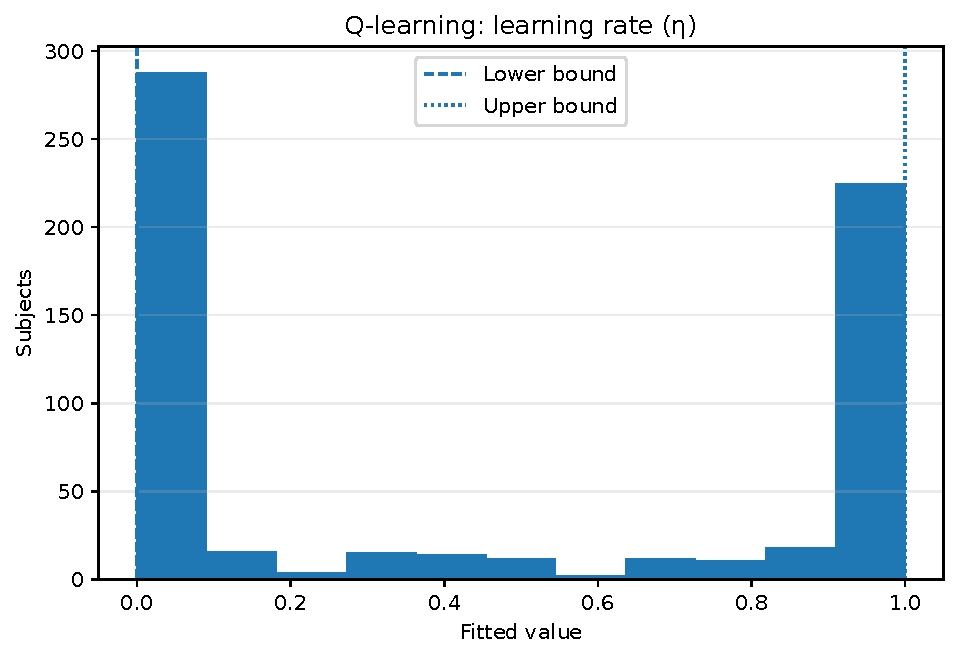
\includegraphics[width=\linewidth]{q_learning_learning_rate_distribution.pdf}
        \caption{Q-learning learning-rate distribution.}
    \end{minipage}\hfill
    \begin{minipage}[t]{0.49\textwidth}\centering
        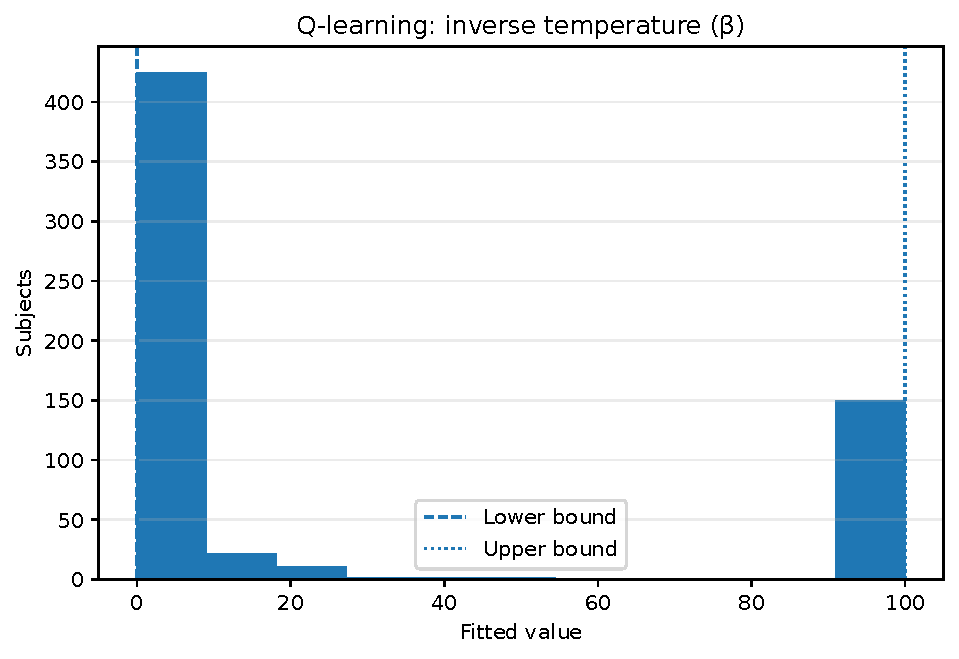
\includegraphics[width=\linewidth]{q_learning_inverse_temperature_distribution.pdf}
        \caption{Q-learning inverse-temperature distribution.}
    \end{minipage}
\end{figure}

\begin{figure}[H]
    \centering
    \begin{minipage}[t]{0.49\textwidth}\centering
        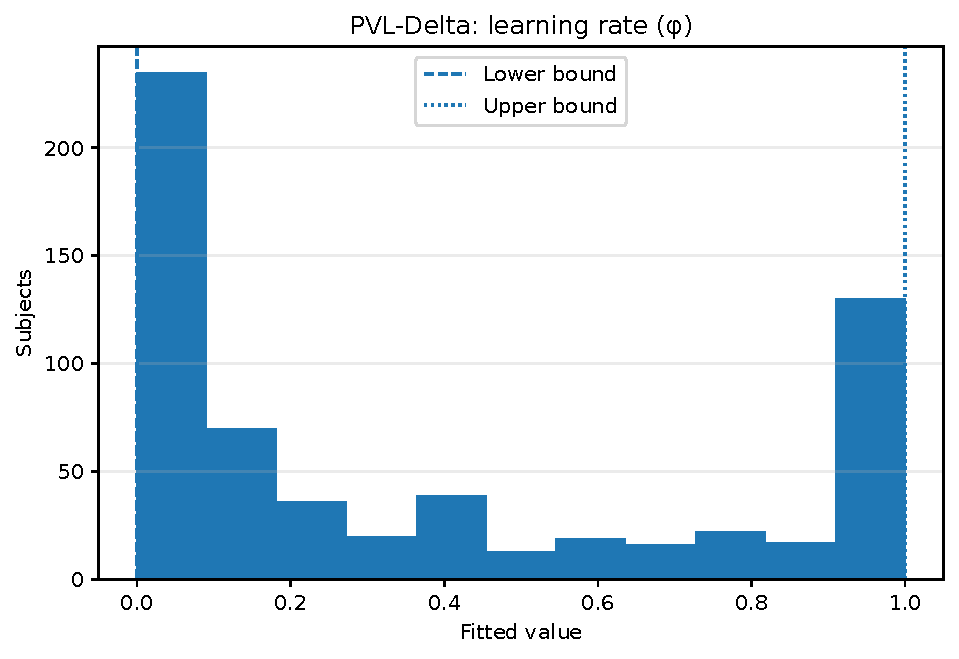
\includegraphics[width=\linewidth]{pvl_delta_learning_rate_distribution.pdf}
        \caption{PVL-Delta learning-rate distribution.}
    \end{minipage}\hfill
    \begin{minipage}[t]{0.49\textwidth}\centering
        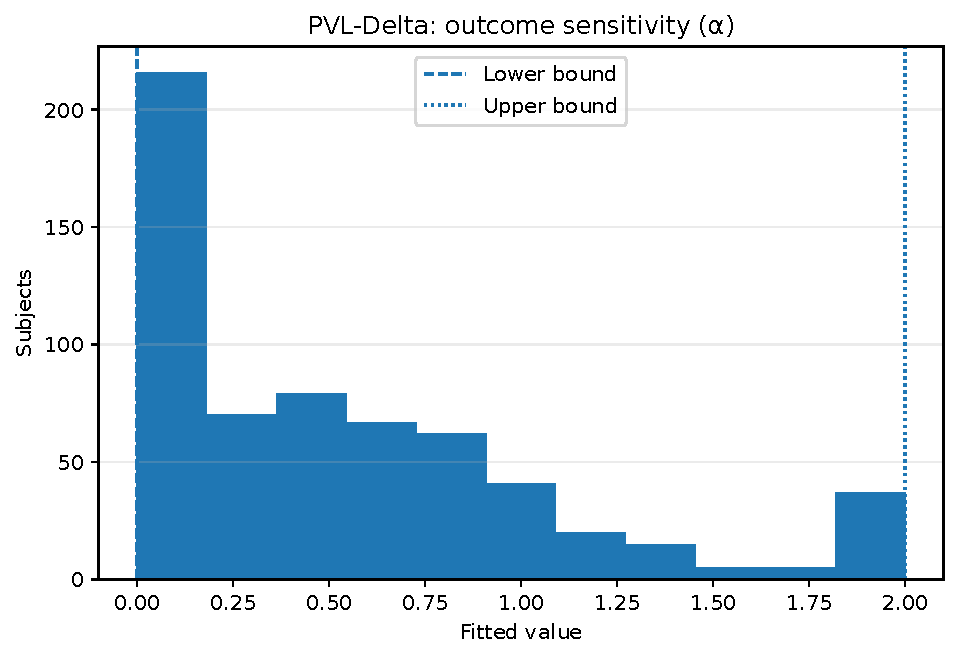
\includegraphics[width=\linewidth]{pvl_delta_outcome_sensitivity_distribution.pdf}
        \caption{PVL-Delta outcome-sensitivity distribution.}
    \end{minipage}
\end{figure}

\begin{figure}[H]
    \centering
    \begin{minipage}[t]{0.49\textwidth}\centering
        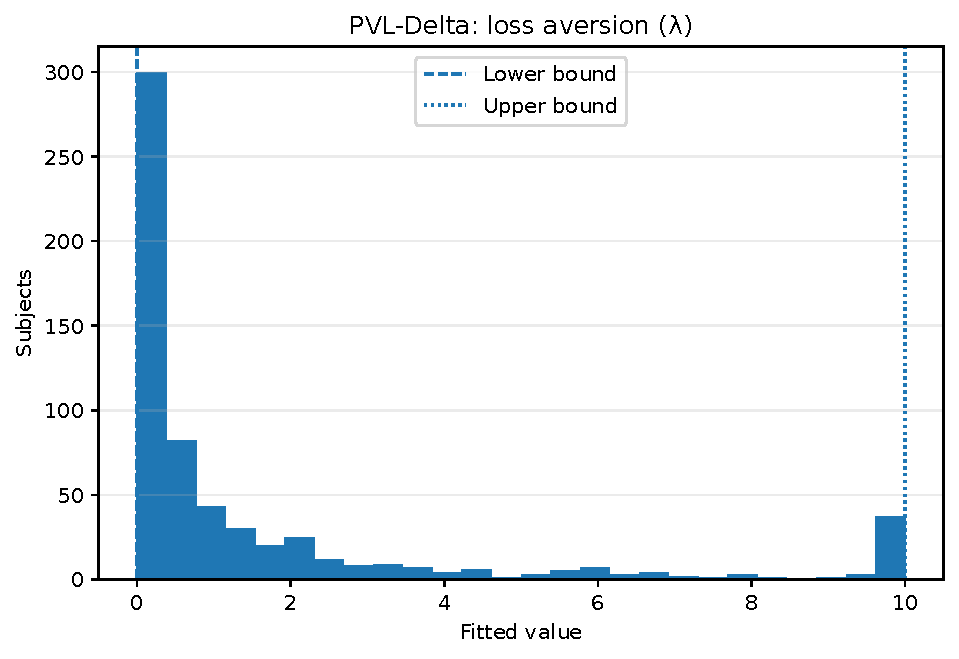
\includegraphics[width=\linewidth]{pvl_delta_loss_aversion_distribution.pdf}
        \caption{PVL-Delta loss-aversion distribution.}
    \end{minipage}\hfill
    \begin{minipage}[t]{0.49\textwidth}\centering
        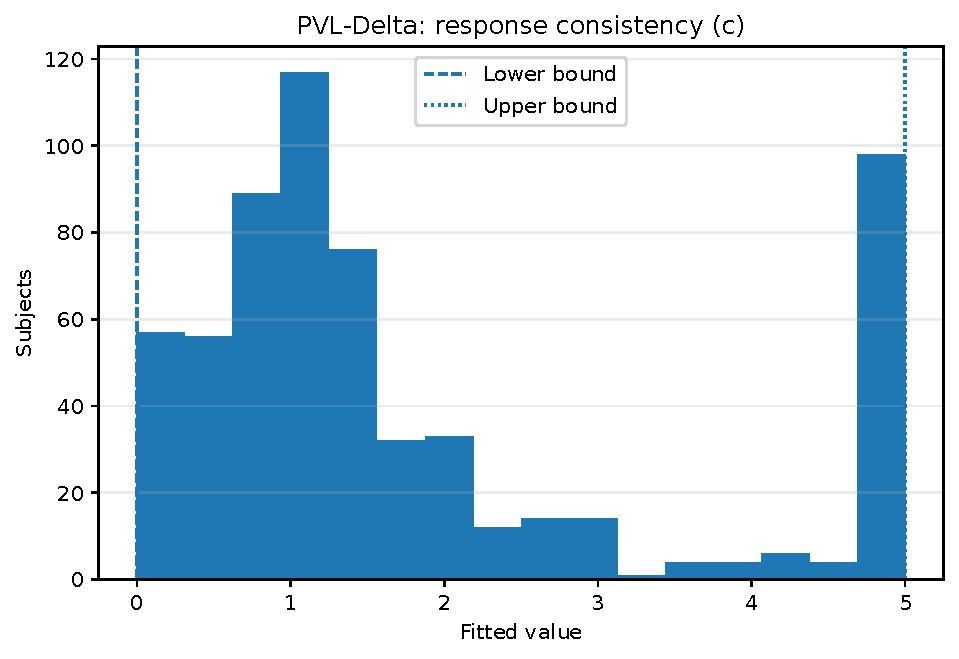
\includegraphics[width=\linewidth]{pvl_delta_response_consistency_distribution.pdf}
        \caption{PVL-Delta response-consistency distribution.}
    \end{minipage}
\end{figure}

\section{Additional Model-Comparison Figures}
\begin{figure}[H]
    \centering
    \begin{minipage}[t]{0.49\textwidth}\centering
        
\includegraphics[width=\linewidth]{q_vs_pvl_aic.pdf}
        \caption{Participant-level AIC comparison.}
    \end{minipage}\hfill
    \begin{minipage}[t]{0.49\textwidth}\centering
        
\includegraphics[width=\linewidth]{q_vs_pvl_bic.pdf}
        \caption{Participant-level BIC comparison.}
    \end{minipage}
\end{figure}

\begin{figure}[H]\centering
\includegraphics[width=0.72\textwidth]{pvl_win_rate_confidence_intervals.pdf}\caption{PVL-Delta model-win rates with exact confidence intervals.}\end{figure}


\end{document}
